\section[Demonstration]{Demonstration}
\label{sec:demonstrations}
\addcontentsline{toc}{section}{\thesection. Demonstrations}
The examples presented below are simulated and are not necessarily
meant to represent meaningful activation study on the brain. Their
purpose is to demonstrate our segmentation methodology in activation
detection. 


\subsection[2D Phantoms]{2D Phantoms}
\label{sec:phantoms}
\addcontentsline{toc}{subsection}{\thesubsection. 2D Phantoms}

Three 2D phantoms built in the \pkg{MixfMRI} package can be displayed in
\proglang{R} 
from the demo as simple as
\begin{Code}[title=Maitra's Phantoms]
R> demo(maitra_phantom, package = "MixfMRI", ask = F)
\end{Code}
which performs the code in \code{MixfMRI/demo/maitra_phantom.r}.
The \proglang{R}
command should give a plot similar to Figure~\ref{fig:maitra_phantom}
containing three different simulated 2D slices of a hypothesized brain.
Each phantom may have different amounts of activated voxels (in terms
of smaller $p$-values). Colors represent different activation intensities.
The total proportions of truly active voxels are listed in the title of
each phantom.
\begin{figure}[h]
\caption{Simulated 2D Phantoms.}
\centering
\vspace{0.2cm}
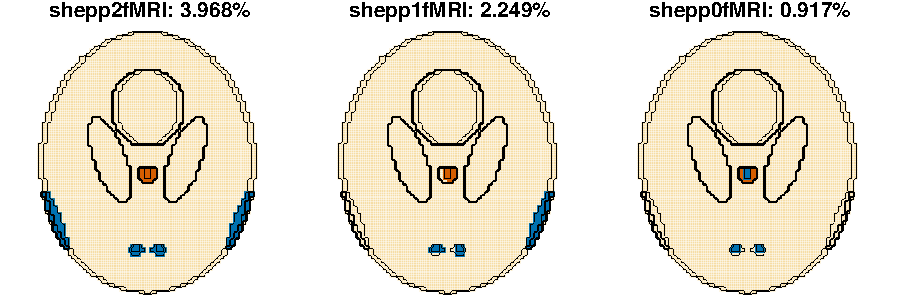
\includegraphics[width=6in]{./MixfMRI-include/maitra_phantom}
\label{fig:maitra_phantom}
\end{figure}

The examples used below mimic some active regions (in 2D)
depending on different types of stimuli that may trigger responses
in the brain.
Hypothetically, the voxels may be active by regions, but
each region may not be active in the same way (or magnitude) even
though they may need to collectively respond to the stimuli (for example, due
to time delay, response order, or sensitivity of study design).

As an example, only 3.968\% of voxels in the \code{shepp2fMRI} phantom are active
and indicated by two different colors (blue and brown)
for different activation types where $p$-values may be smaller than 0.05
and may follow two Beta distributions (with different configurations)
for the truly active voxels and one uniform distribution (i.e. $Beta(1, 1)$)
for the truly inactive voxels.

The following code provides some counts for each groups of active and
inactive voxels in the \code{shepp2fMRI} phantom.
\begin{CodeOutput}[title=Summary of shepp2fMRI Phantoms]
> table(shepp2fMRI, useNA="always")
shepp2fMRI
    0     1     2  <NA> 
13408   472    82 51574 
\end{CodeOutput}
The summary says that this phantom has three kinds of activations
with group ids: 0, 1, and 2.
There are 13,408 voxels belonging to cluster 0 (inactive),
followed by 472 voxels belonging to cluster 1 (active \& highlighted in
blue in Figure~\ref{fig:maitra_phantom}), and
82 voxels belonging to cluster 2 (active \& high lighted in
 brown in Figure~\ref{fig:maitra_phantom}).
There are 51,574 pixels (NA) of this
imaging dataset which are not within the brain (contour by the black line
in Figure~\ref{fig:maitra_phantom}).
See Section~\ref{sec:2d_simulations} for information of generating
p-values from a mixture of three Beta distributions.


\subsection[2D Simulations]{2D Simulations}
\label{sec:2d_simulations}
\addcontentsline{toc}{subsection}{\thesubsection. 2D Simulations}

The \pkg{MixfMRI} provides a function \code{gendataset(phantom, overlap)}
to generate p-values of activations.
The function needs two arguments: \code{phantom} and \code{overlap}.
The \code{phantom} is a map containing voxel group id's
where p-values will be simulated from a mixture Beta distribution with
certain mixture level specified by the \code{overlap} argument.
The example can be found in
\code{MixfMRI/demo/maitra_2d.r} and can be done in \proglang{R}
as simple as
\begin{Code}[title=Simulations of Active Voxels]
R> demo(maitra_2d, package = "MixfMRI", ask = F)
\end{Code}
Note that the overlap repesents similarity of activation signals. The higher
the overlap, the more difficult it becomes to distinguish between
activation and inactivation and also the kinds of activation. 

The command above should give a plot similar to Figure~\ref{fig:maitra_2d}
containing group id's on the left and their associated
p-values for stimulus responses on the right.
The top row displays examples for phantom \code{shepp1fMRI}, and the
bottom row displays examples for phantom \code{shepp2fMRI}.
\begin{itemize}
\item
Inside the brain,
the group id 2's are indicated by white (active is highly associated with
stimula due to experiment design),
1's are indicated by light gray (slightly active),
and 0's are indicated by dark gray (inactive).
Note that the region with white color was the region colored  blue
and the light gray region corresponds to the region colored brown in
Figure~\ref{fig:maitra_phantom} 
\item
The simulated $p$-values are colored by a map using  a
red-orange-yellow palette from 0 to 1.
Note that small $p$-values (redder voxels) may also occur at truly inactive voxels.
\end{itemize}
See Figure~\ref{fig:maitra_2d_fclust} for the distribution of
simulated p-values for the phantom \code{shepp2fMRI}.

\begin{figure}[h]
\caption{Activated regions of voxels and simulated $p$-values.}
\centering
\vspace{0.2cm}
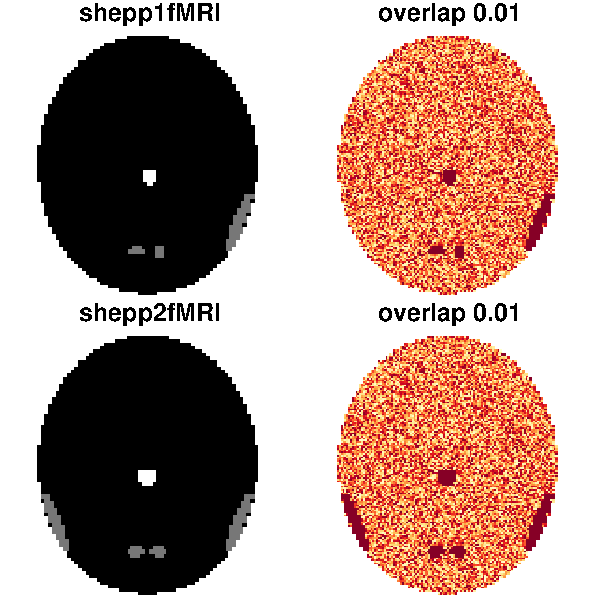
\includegraphics[width=4in]{./MixfMRI-include/maitra_2d}
\label{fig:maitra_2d}
\end{figure}

The methodology and analyses implemented in this package aim to 
identify those active voxels in spatial clusters. For example,
regions of active voxels associated with imagining the playing of certain
sports. 
When an experiment was conducted/designed to detect brain behaviors,
the statistical model and the $p$-values of the treatment effect
should be able to reflect the voxel activations.
Typically, the statistical tests are done independently voxel-by-voxel
due to complexity of computation and modeling.
This package provides post hoc clustering that adds spatial contents
to p-values and helps to isolate meaningful regions
clouded with many small $p$-values.
See \cite{ChenMaitra2018} for information of clustering performance and
comprehensive assessments for this post hoc approach.


\subsection[2D Clustering]{2D Clustering}
\addcontentsline{toc}{subsection}{\thesubsection. 2D Clustering}

The example can be found in
\code{MixfMRI/demo/maitra_2d_fclust.r} as simple as
\begin{Code}[title=Clustering of Active Voxels]
R> demo(maitra_2d_fclust, package = "MixfMRI", ask = F)
\end{Code}
This demo (explained below) is to cluster the simulated $p$-values
(see Section~\ref{sec:2d_simulations}) using the developed method.
\begin{Code}[title=Code of \code{maitra\_2d\_fclust.r}]
library(MixfMRI, quietly = TRUE)
set.seed(1234)
da <- gendataset(phantom = shepp2fMRI, overlap = 0.01)$pval

### Check 2d data.
id <- !is.na(da)
PV.gbd <- da[id]
# pdf(file = "maitra_2d_fclust.pdf", width = 6, height = 4)
hist(PV.gbd, nclass = 100, main = "p-value")
# dev.off()

### Test 2d data.
id.loc <- which(id, arr.ind = TRUE)
X.gbd <- t(t(id.loc) / dim(da))
ret <- fclust(X.gbd, PV.gbd, K = 3)
print(ret)

### Check performance
library(EMCluster, quietly = TRUE)
RRand(ret$class, shepp2fMRI[id] + 1)
\end{Code}
In the code above, the histogram of simulated $p$-values is plotted in
Figure~\ref{fig:maitra_2d_fclust}.
Then, the
\code{fclust(X.gbd, PV.gbd, K = 3)} groups voxels in three clusters.
At the end, \code{ret} saves the clustering results.
The \code{print(ret)} from the above code will show the results below
in detail:
\begin{itemize}
\item \code{N} is the total number of voxels to be clustered/segmented
\item \code{K} is the total number of segments.
\item \code{n.class} is the number of voxels in each segment
\item \code{ETA} is the mixing proportion of each segment
\item \code{BETA} is the set of parameters of the Beta distributions
  (by column) 
\item \code{MU} is the centers of the segements (the spatial location
  inside the brain) 
\item \code{SIGMA} is the dispersion of the segments
\end{itemize}

\begin{figure}[h]
\caption{Activation ($p$-values) Distribution. The x-axis is for the p-values.}
\centering
\vspace{0.2cm}
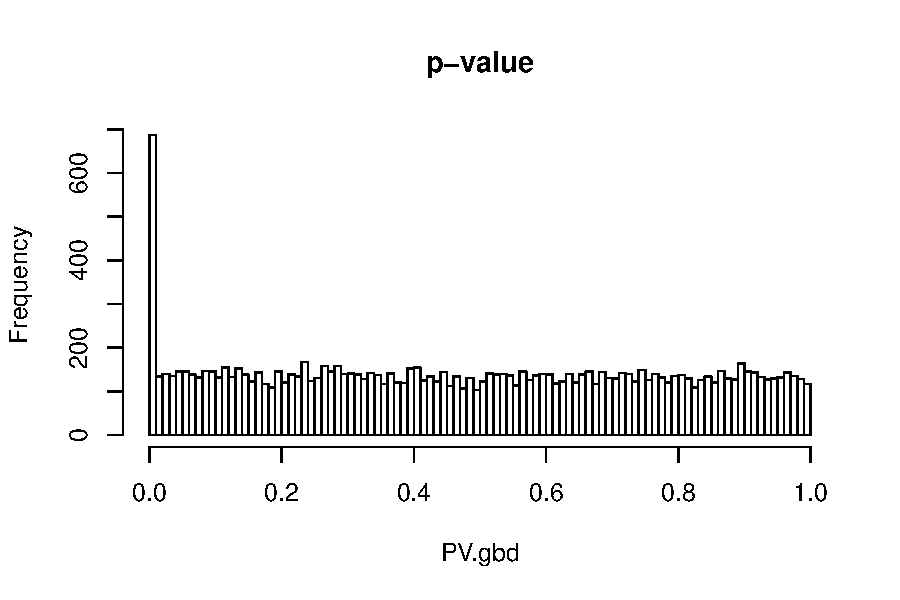
\includegraphics[width=6in]{./MixfMRI-include/maitra_2d_fclust}
\label{fig:maitra_2d_fclust}
\end{figure}

The numbers of voxels for each segment, in this example, are
13,394, 184, and 384 associated with new cluster ids: 0, 1, and 2,
respectivelly.
Comparing with the true classifications (see the table in
Section~\ref{sec:phantoms}), the adjusted Rand index gives
$0.9749$ indicating good agreement between the truly active and the
activated (as determined by our segmentation methodology) results. 

\begin{CodeOutput}[title=Outputs of Clustering]
R> print(ret)
Algorithm: apecma  Model.X: I  Ignore.X: FALSE
- Convergence: 1  iter: 16  abs.err: 0.02091979  rel.err: 7.375343e-07
- N: 13962  p.X: 2  K: 3  logL: 28364.52
- AIC: -56693.04  BIC: -56557.25 ICL-BIC: -55712.18
- n.class: 13394 184 384
- init.class.method: 
- ETA: (min.1st.prop: 0.8  max.PV: 0.1)
[1] 0.95266704 0.01307847 0.03425449
- BETA: (2 by K)
     [,1]         [,2]       [,3]
[1,]    1 1.127244e-01 0.04237128
[2,]    1 4.429518e+04 1.00000130
- MU: (p.X by K)
          [,1]      [,2]      [,3]
[1,] 0.5013538 0.3105460 0.5917377
[2,] 0.5076080 0.3718145 0.3749842
- SIGMA: (d.normal by K)
           [,1]         [,2]        [,3]
[1,] 0.01271198 0.0001859628 0.009462210
[2,] 0.02186662 0.0011582052 0.004284016

R> RRand(ret$class, shepp2fMRI[id] + 1)
   Rand adjRand  Eindex 
 0.9964  0.9749  1.7012 
\end{CodeOutput}

